\section{Cámara}
\label{section:camara}

Este proyecto integra una cámara conocida como M5 Stack Timercam \footnote{M5 Stack Timercam \url{https://m5stack.com/products/timercam-m5stack}}, que destaca por su capacidad para realizar streaming de las imágenes captadas vía HTTP. Además, está equipada con un software de detección de códigos QR.

La cámara M5 Stack Timercam es fundamental en este proyecto debido a su capacidad para proporcionar una retroalimentación visual en la interfaz de usuario. El sistema de apuntado se beneficia de un componente que reacciona si se ha logrado un apuntado correcto, permitiendo al usuario percibir de manera clara si están funcionando correctamente sus interacciones con la interfaz (véase la figura \ref{figure:camera})

\begin{figure}[!htb]
   \centering
    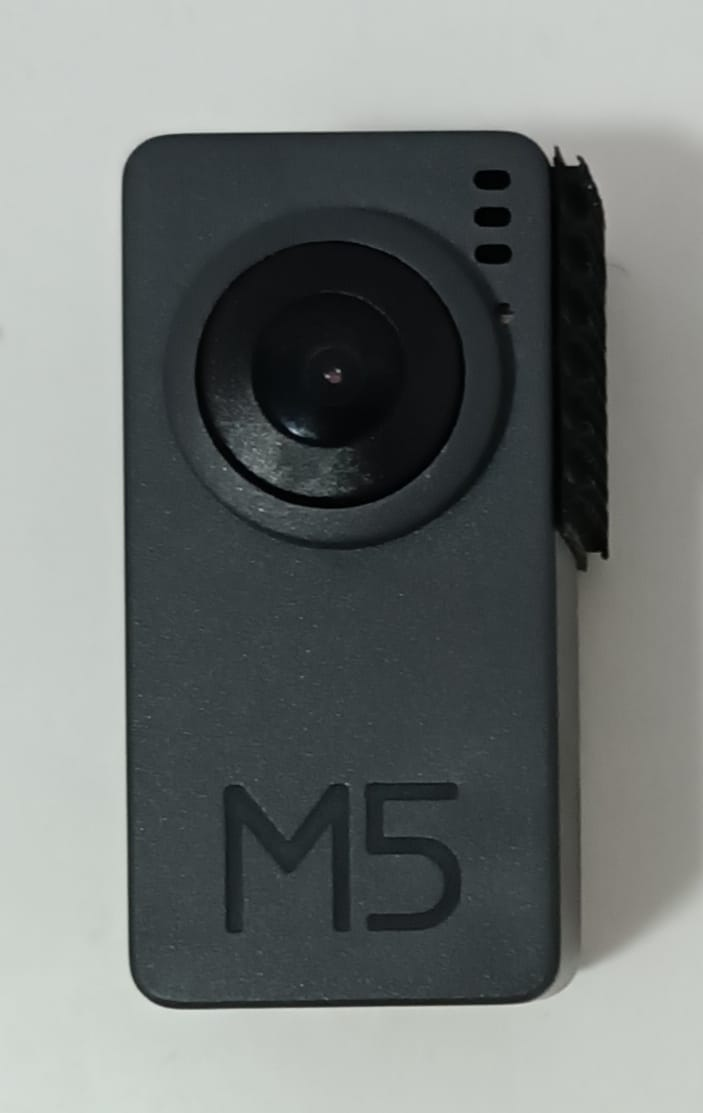
\includegraphics[width=0.25\linewidth]{figures/camera.jpg}
   \caption{Cámara M5 Stack Timercam}
   \label{figure:camera}
\end{figure}

